\chapter{Image processing and tracking of all the cells in the given $\textbf{\textit{E.coli}}$ movie using u-track 2.0, and perform data analysis} % Main chapter title

\label{Part1_chapter} % For referencing the chapter elsewhere, use \ref{Chapter1} 

\section{Get data form movie}
 
For the video: 1 pixel = 0.65 $\mu m$, 1 frame = 0.1 second.\\
The data were extracted by u-track to track the cell by method of Single-Particles and Gaussian Mixture-model Fitting. There are more than 14000 tracks.

\newpage
\section{Single bacteria trajectory}

Form 14721 tracks, I chose the track with the biggest number of un-NAN values and removed all of the NAN value to plot the movement of this single bacteria. 

%----------------------------------------------------------------------------------------

\begin{figure}[H]
\centering
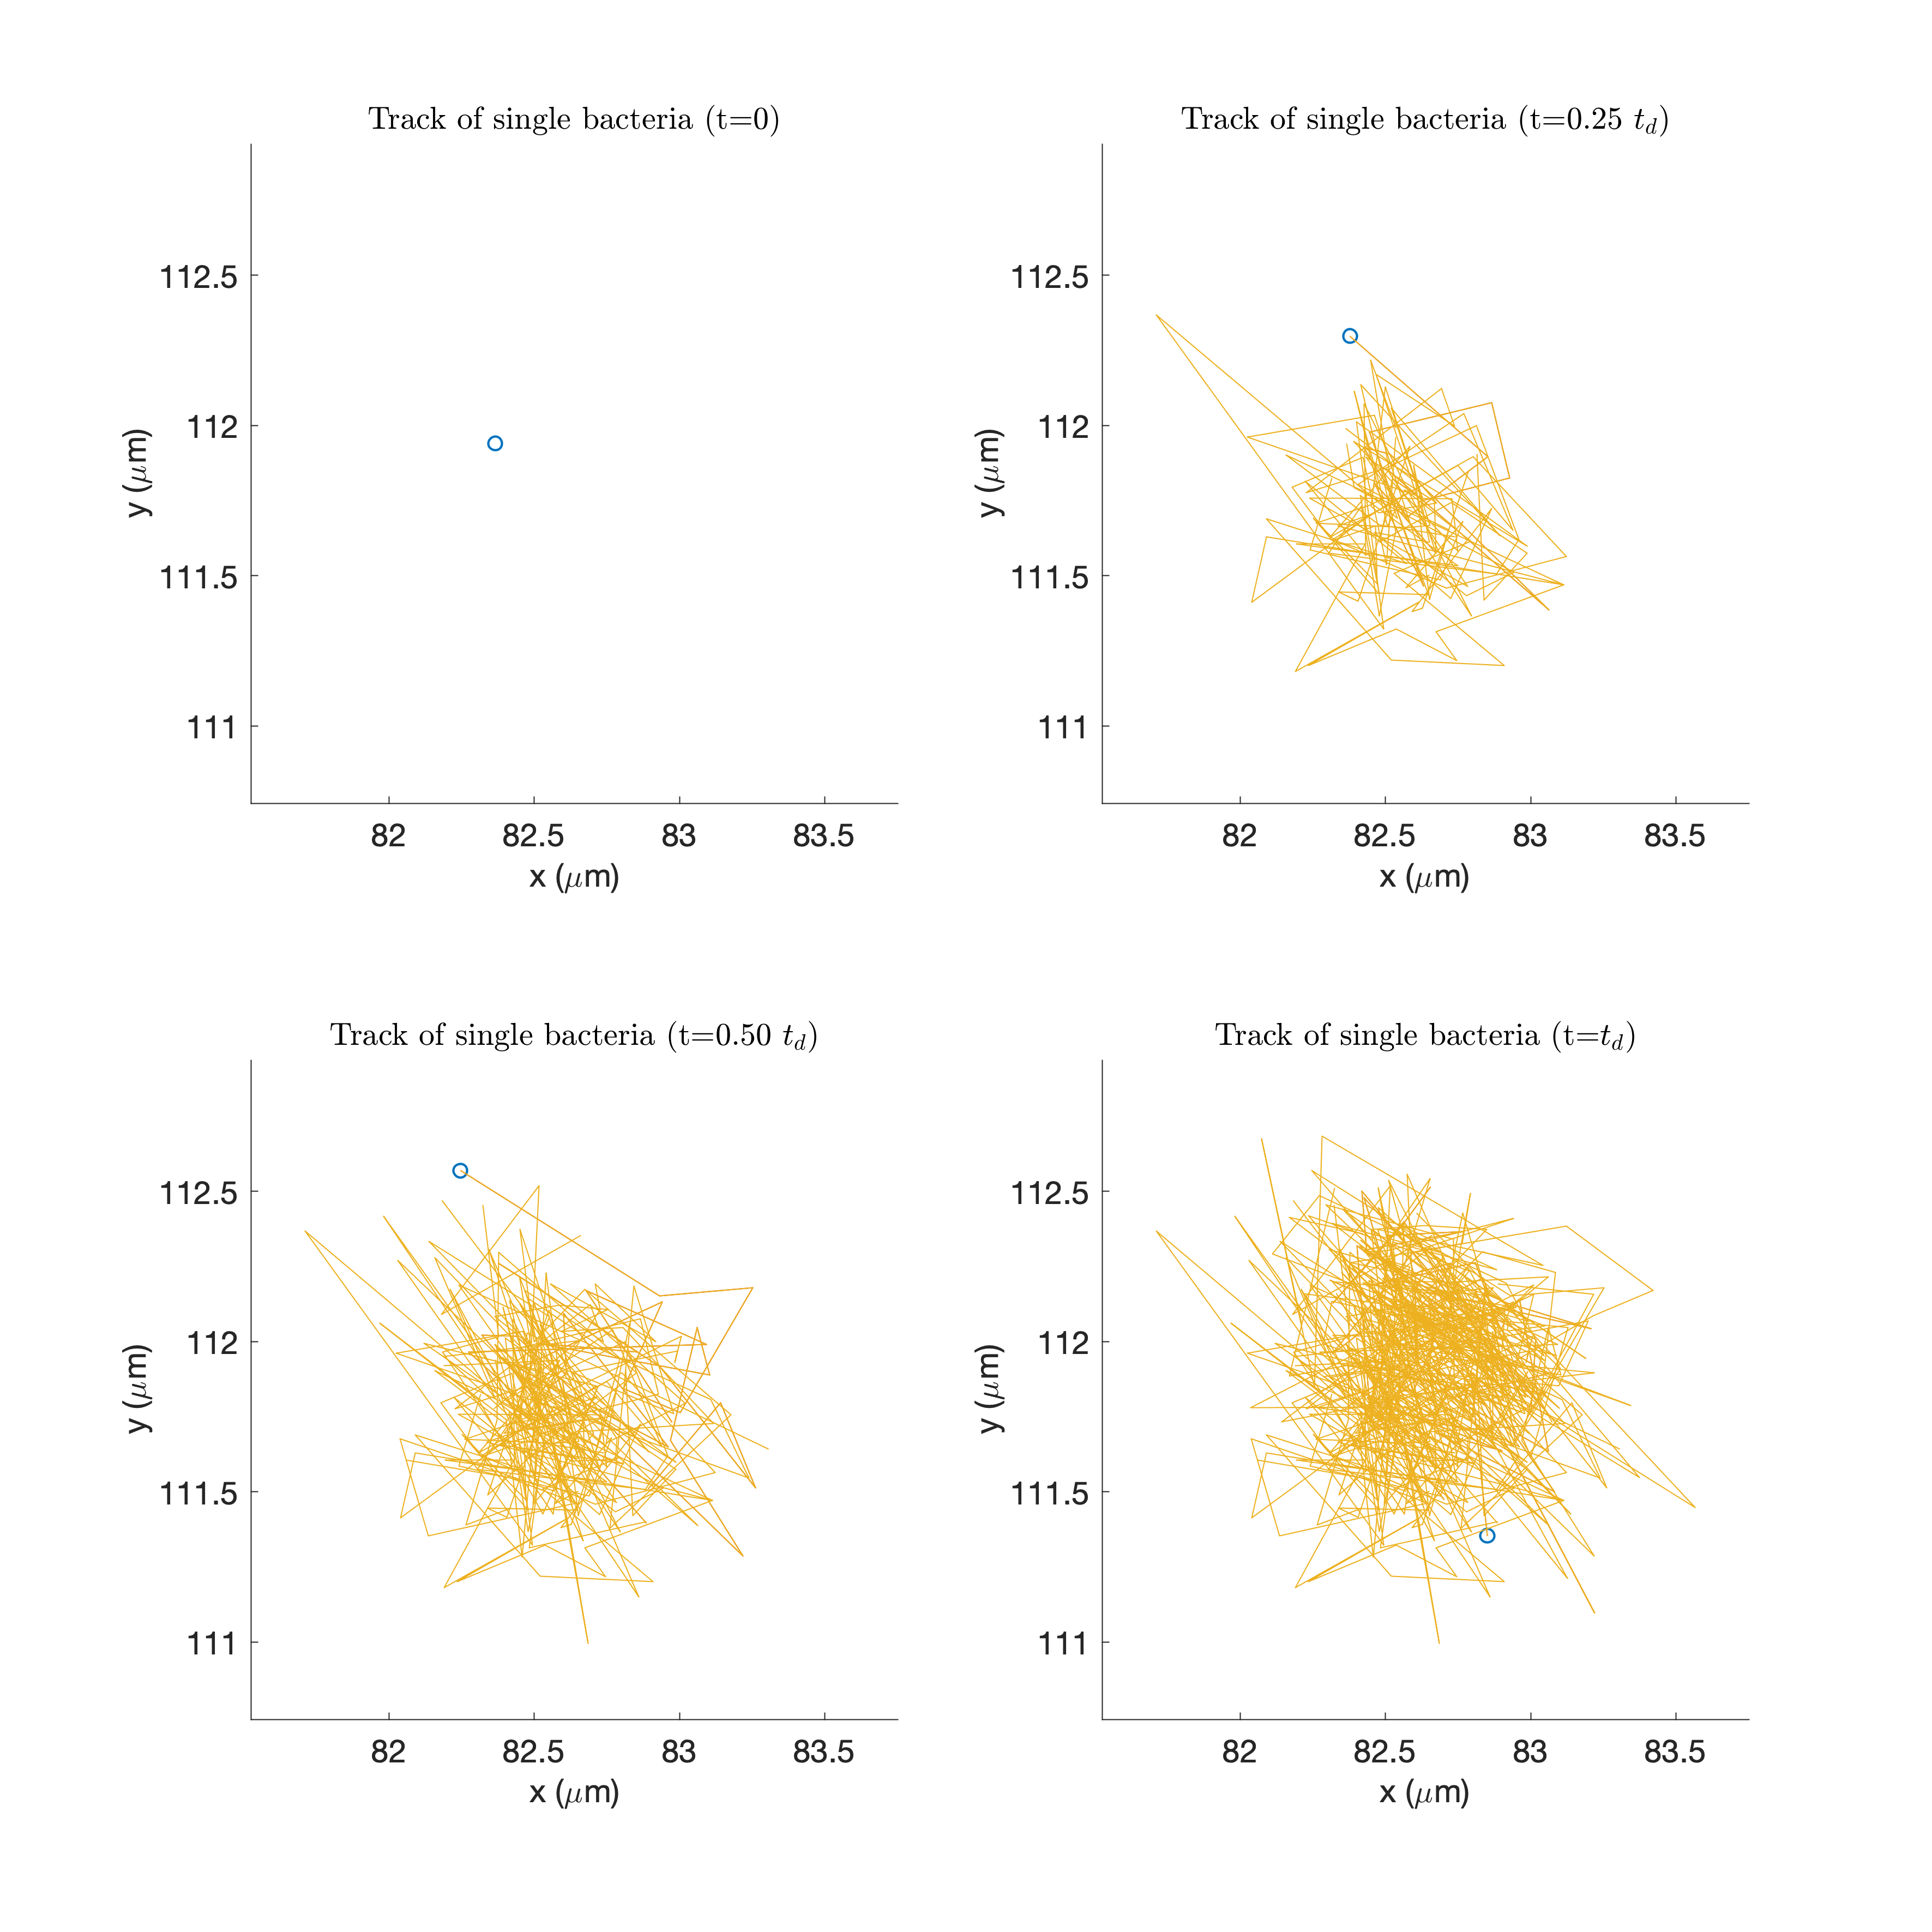
\includegraphics[width=1\linewidth]{Figures/P3_fig1.png}
\caption{Single Bacteria Random Walk Trajectory}
\label{P2_fig1}
\end{figure}

\section{Bacteria population trajectory}
Also track all the cells from the data, to calculate the population motions. The statistical results are shown in Figure 3.2.
\begin{figure}[H]
\centering
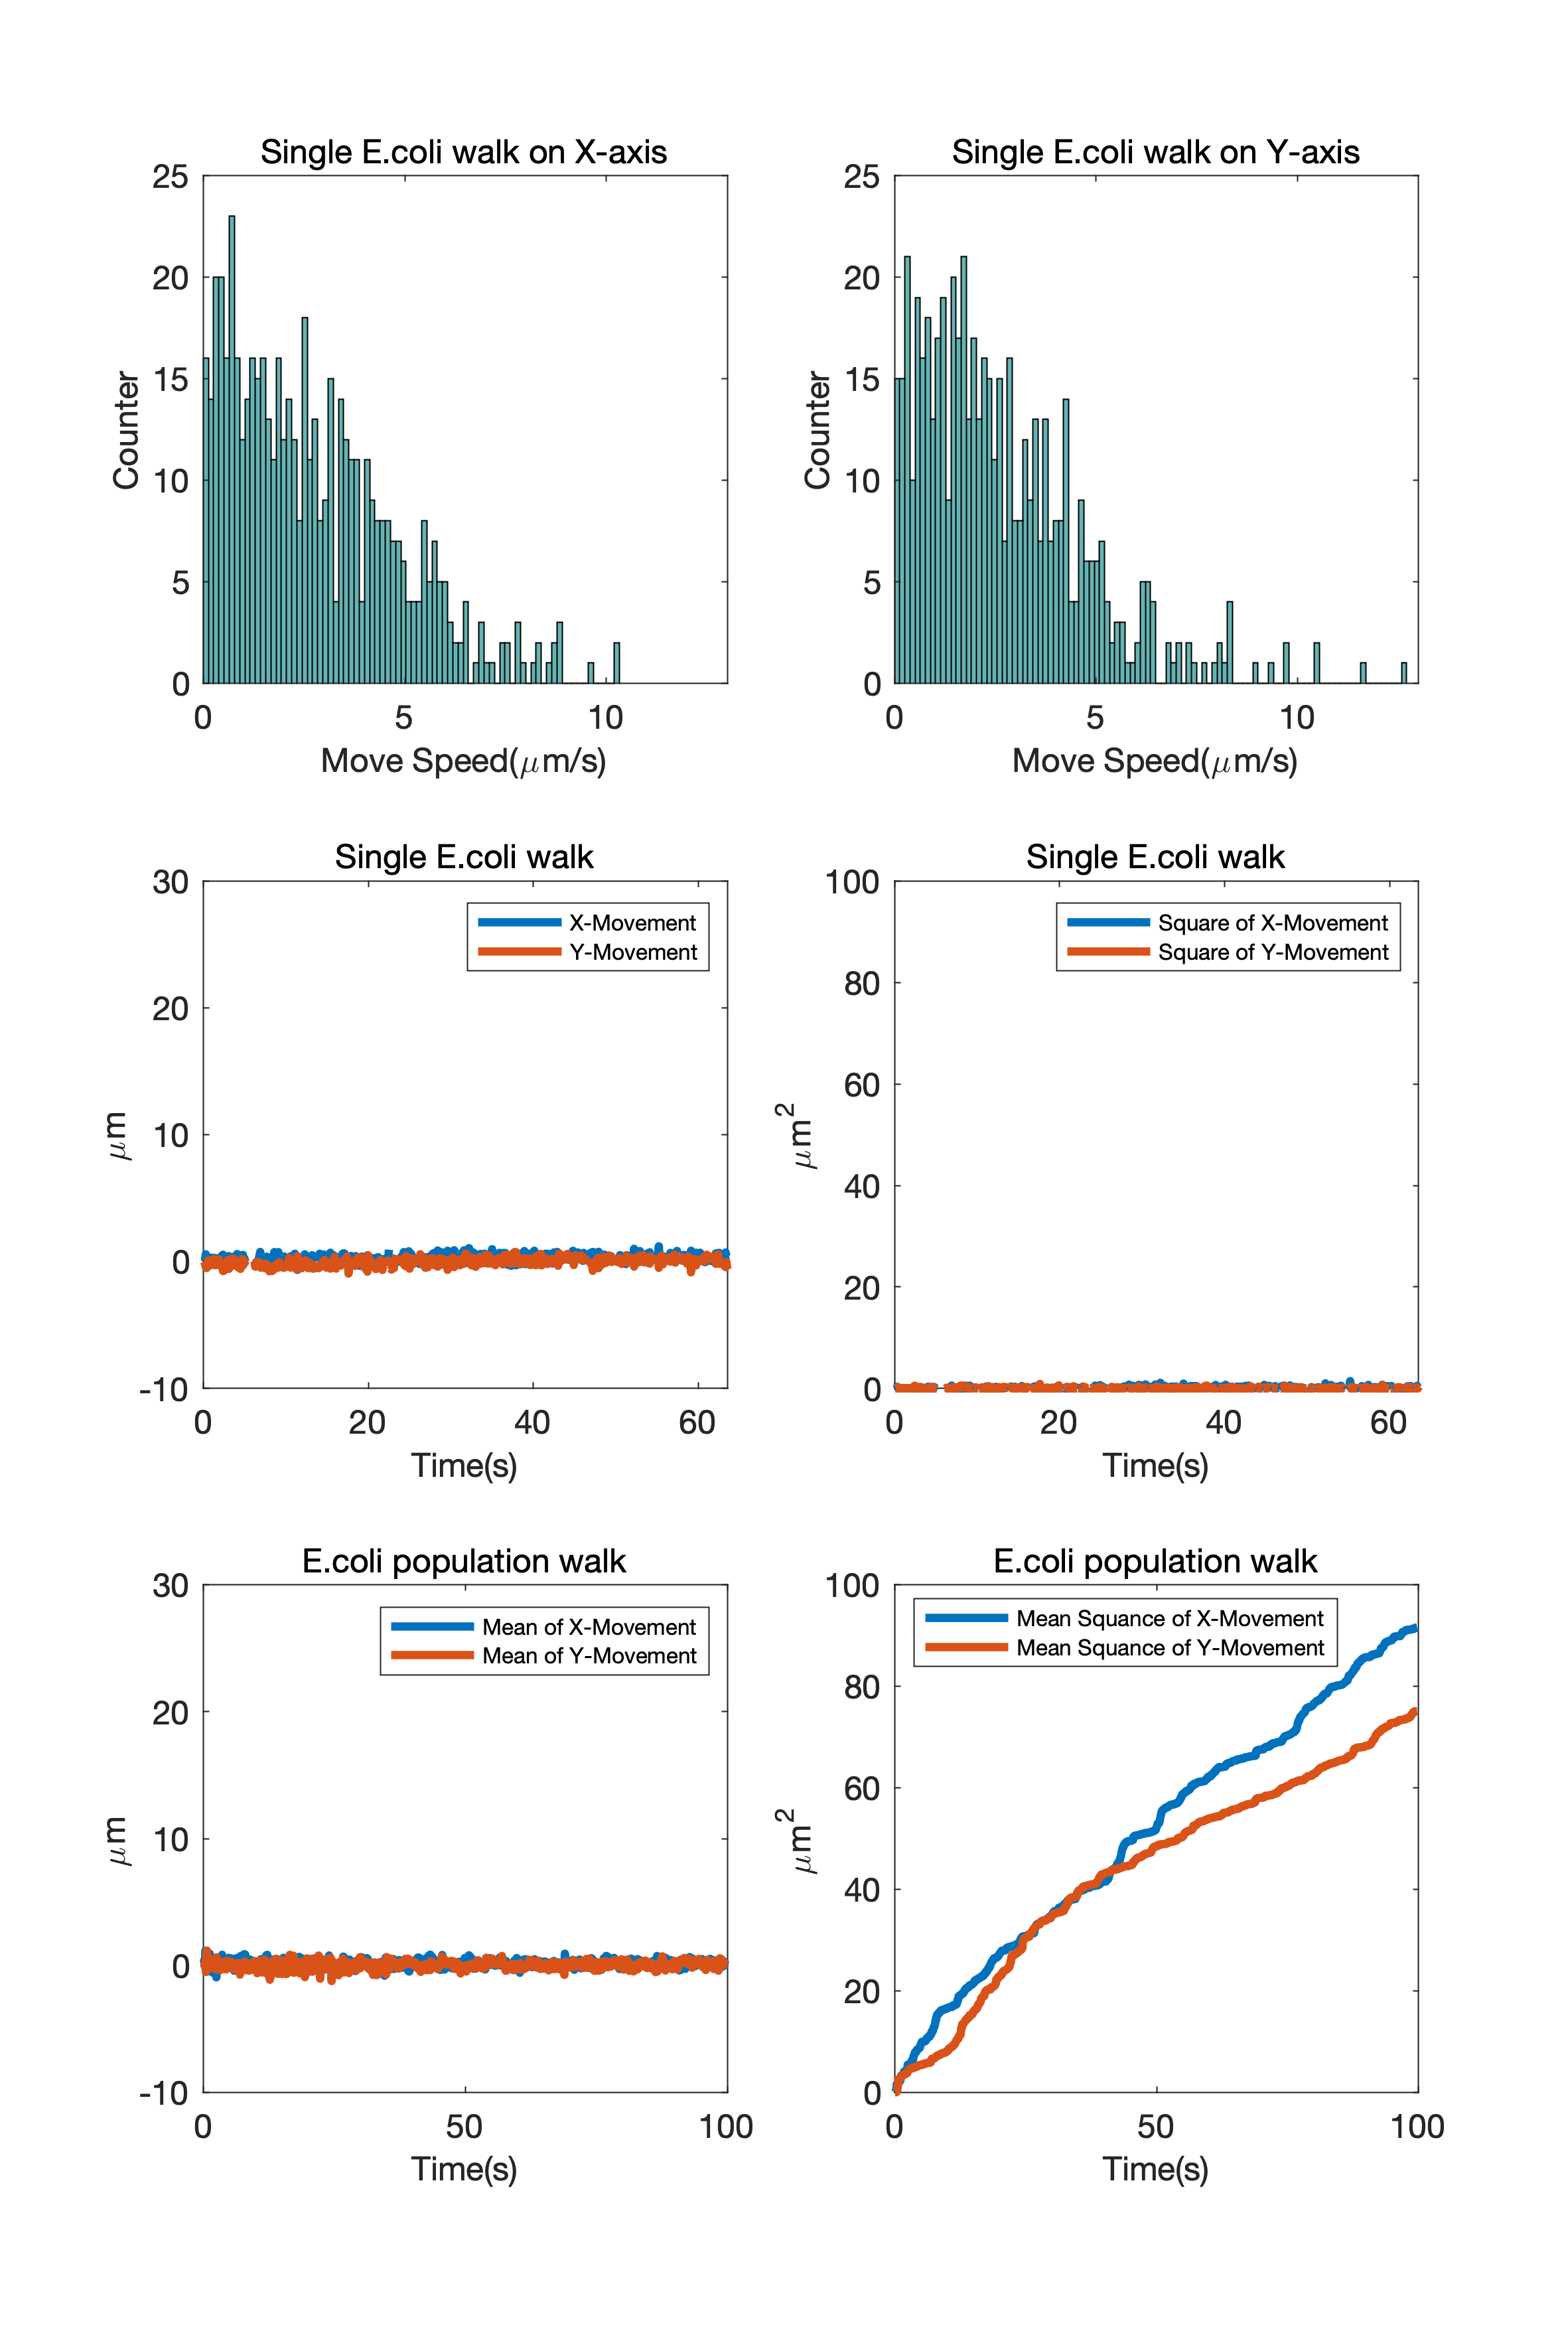
\includegraphics[width=0.75\linewidth]{Figures/P3_fig2.png}
\caption{The ``mean displacement'' and ``mean displacement-square'' overtime for the cells in vedio}
\label{P2_fig2}
\end{figure}

\section{Fitting the Data with the Model}
For a series of scatter points $(x_i, y_i)(i=1,2,...,n)$, if a direct proportional function was used to fit the data, we have:\\
\begin{equation*} 
\begin{aligned} 
\centering
y     &= \beta x \\
\beta &= \sum_{i=1}^n x_i y_i \Big / \sum_{i=1}^n x_i^2 \\
\end{aligned} 
\end{equation*}
As for our model: \\
\begin{equation*} 
\begin{aligned} 
\centering
\frac{1}{n} \sum_{i=1}^{n}x_i(t)^2 &= v_x^2t \\
\frac{1}{n} \sum_{i=1}^{n}y_i(t)^2 &= v_y^2t \\
\end{aligned} 
\end{equation*}
So there are the fitting model: \\
\begin{equation*} 
\begin{aligned} 
\centering
\frac{1}{n} \sum_{i=1}^{n}x_i(t)^2 &= \beta_x t = v_x^2t \\
\frac{1}{n} \sum_{i=1}^{n}y_i(t)^2 &= \beta_y t = v_y^2t \\
\beta_x = \sum_{i=1}^n & t_i x_i \Big / \sum_{i=1}^n t_i^2 \\
\beta_y = \sum_{i=1}^n & t_i y_i \Big / \sum_{i=1}^n t_i^2 \\
\end{aligned} 
\end{equation*}
We get: \\
\begin{equation*} 
\begin{aligned} 
\centering
\beta_x &= 0.9862 \mu m^2 /s^2 \\
v_x &= 0.9931 \mu m /s \\
\beta_y &= 0.8366 \mu m^2 /s^2 \\
v_y &= 0.9147 \mu m /s \\
\end{aligned} 
\end{equation*}
%betaX = 0.9862
%betaY = 0.8366
\begin{figure}[H]
\centering
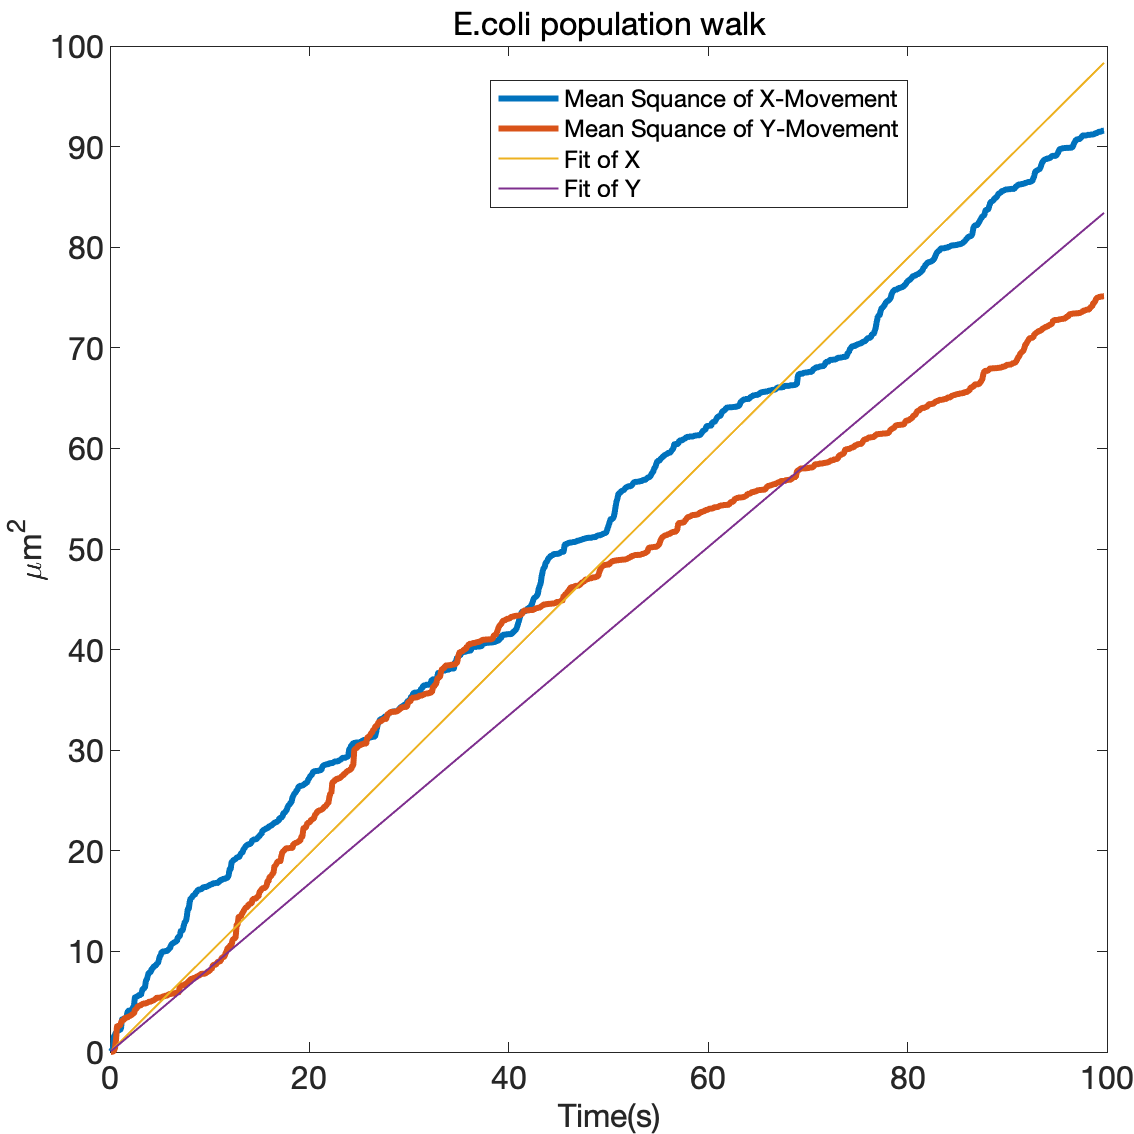
\includegraphics[width=1\linewidth]{Figures/P3_fig3.png}
\caption{Fitting the Data by Model}
\label{P3_fig3}
\end{figure}
%----------------------------------------------------------------------------------------



%----------------------------------------------------------------------------------------




%The \code{biblatex} package is used to format the bibliography and inserts references such as this one \parencite{Reference1}. The options used in the \file{main.tex} file mean that the in-text citations of references are formatted with the author(s) listed with the date of the publication. Multiple references are separated by semicolons (e.g. \parencite{Reference2, Reference1}) and references with more than three authors only show the first author with \emph{et al.} indicating there are more authors (e.g. \parencite{Reference3}). This is done automatically for you. To see how you use references, have a look at the \file{Chapter1.tex} source file. Many reference managers allow you to simply drag the reference into the document as you type.

